\subsection{Scenari}
	\subsubsection{Gestione richiesta di registrazione}
	Il seguente diagramma rappresenta lo scenario con il quale viene gestita una richiesta di registrazione. La richiesta viene gestita da \textit{RegistrationController} che controlla il corretto inserimento dei dati e invia il responso a \textit{UsersController}, il quale può agire in due modi diversi: se la richiesta é stata fatta correttamente allora invia un CreateUser() a Utenti per creare il nuovo utente, avvisa \textit{RegistrationController} che la registrazione é avvenuta tramite RegistrationDone() e viene emanato un segnale di Redirect(); se la richiesta ha prodotto degli errori viene inviato un RegistrationError() a \textit{RegistrationController} che comunica l'errore per mezzo di un ErrorMessage().
	\begin{figure}[H]
		\centering
		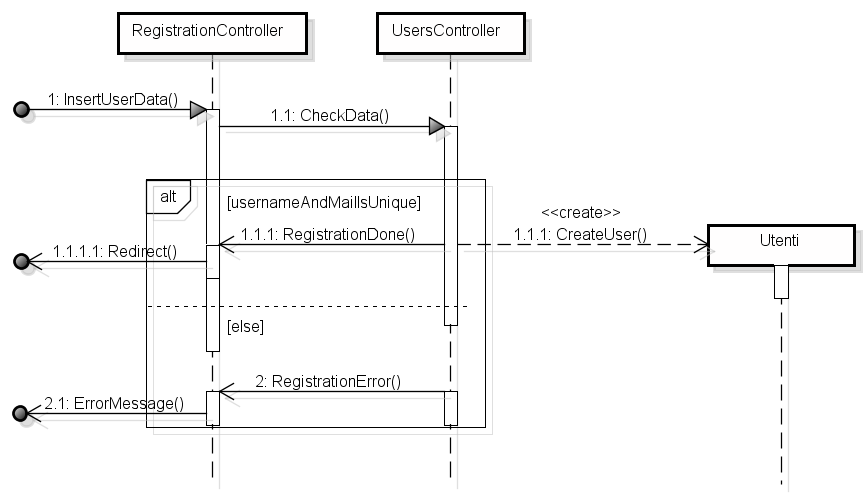
\includegraphics[scale=0.5]{img/register.png}
		\caption{Diagrammi di sequenza - Richiesta di registrazione}
	\end{figure}

\newpage
	\subsubsection{Gestione richiesta di autenticazione}
	Il seguente diagramma rappresenta lo scenario con il quale viene gestita una richiesta di autenticazione. La richiesta viene presa in carico da \textit{LoginController} che verifica i dati e invia un CheckData() a \textit{UsersController}, da qui viene inviato un SearchForUser() a \textit{Utenti} per trovare una corrispondenza. Se le credenziali sono corrette \textit{Utenti} lo segnala a \textit{UsersController} tramite CorrectCredentials() e alla fine viene emesso un segnale di Redirect(); se le credenziali non sono corrette viene segnalato l'errore con un IncorrectCredentials() e in uscita arriva un ErrorMessage().\\
	Da qui è possibile che arrivi una richiesta di recupero password. Essa é gestita da \textit{LoginController} che invia un CredentialsRecoveryRequest() a \textit{ForgotPasswordController}, poi \textit{UsersController} verifica i dati ricevuti e ricerca l'utente con un SearchForUser() verso \textit{Utenti}. Se i dati per il recupero password sono corretti \textit{UsersController} invia un CredentialsSendToMail() a \textit{ForgotPasswordController}, altrimenti viene inviato un CredentialsError(). Alla fine inviato un segnale in uscita RecoveryMessage() o ErrorMessage() da \textit{LoginController} rispettivamente se il recupero credenziali ha avuto buon esito o se é fallito.

	\begin{figure}[H]
		\centering
		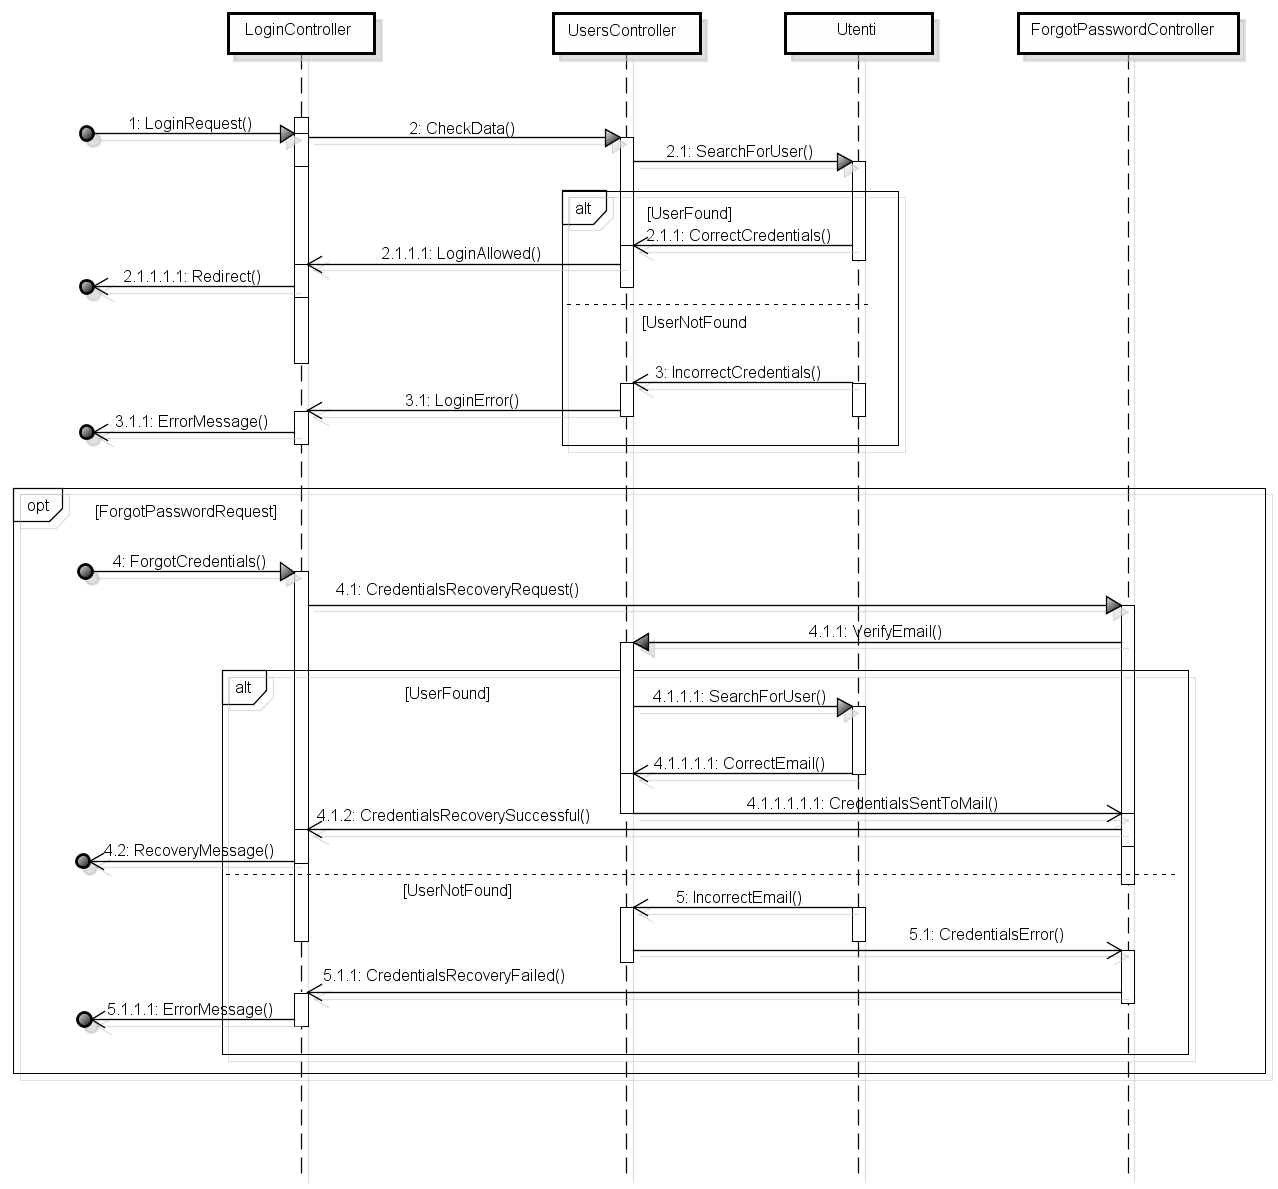
\includegraphics[width=0.9\textwidth]{img/login.png}
		\caption{Diagrammi di sequenza - Richiesta di autenticazione}
	\end{figure}

\newpage
	\subsubsection{Gestione richiesta di ricerca di un progetto}
	Il diagramma seguente rappresenta lo scenario con il quale viene gestita una richiesta di ricerca di un progetto. \textit{SearchResultController} interpreta la richiesta e definisce se sia una ricerca tramite nome utente o tramite nome del progetto. Nel primo caso viene inviato un CheckData() a \textit{UsersController} che verifica la richiesta e invia un SendResults() a \textit{SearchResultsController} che emette un DataResults(). Nel secondo caso il CheckData() viene inviato a \textit{ProjectController} che risponde con un SendResults() a \textit{SearchResultsController} che invia un DataResults().
	\begin{figure}[H]
		\centering
		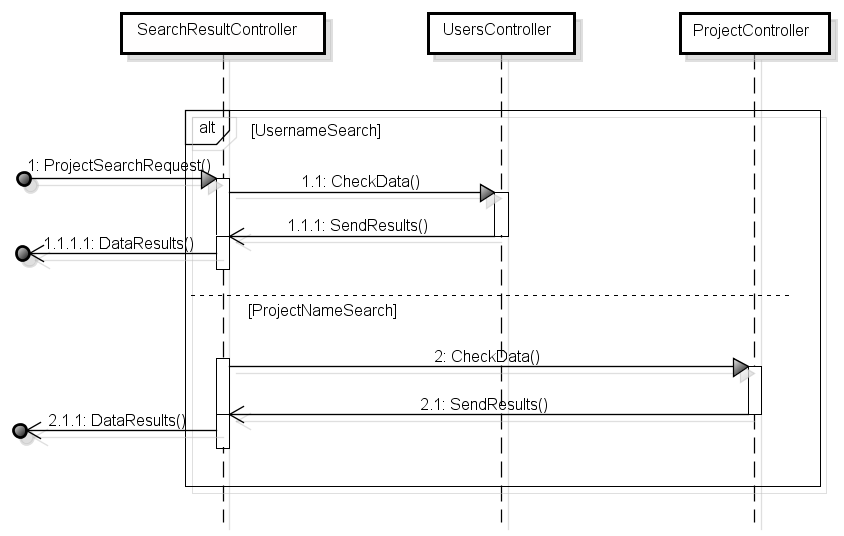
\includegraphics[scale=0.5]{img/search.png}
		\caption{Diagrammi di sequenza - Richiesta di ricerca di un progetto}
	\end{figure}
	
\newpage	
	\subsubsection{Gestione richiesta di visualizzazione di una presentazione}
	Il diagramma seguente rappresenta lo scenario con il quale viene gestita una richiesta di visualizzazione di una presentazione. La richiesta é gestita da \textit{PresentationController} che invia un FindPresentation() a \textit{Presentation} che recupera la prima \gls{slide} tramite un RetrieveFirstSlide() verso \textit{\gls{Slide}}, il quale ritorna un FirstSlideFound(). Infine \textit{Presentation} segnala a \textit{PresentationController} che la visualizzazione é pronta, viene inviato un ViewingReady() a \textit{PresentationController} che ritorna un ViewingStartData().
	
	\begin{figure}[H]
		\centering
		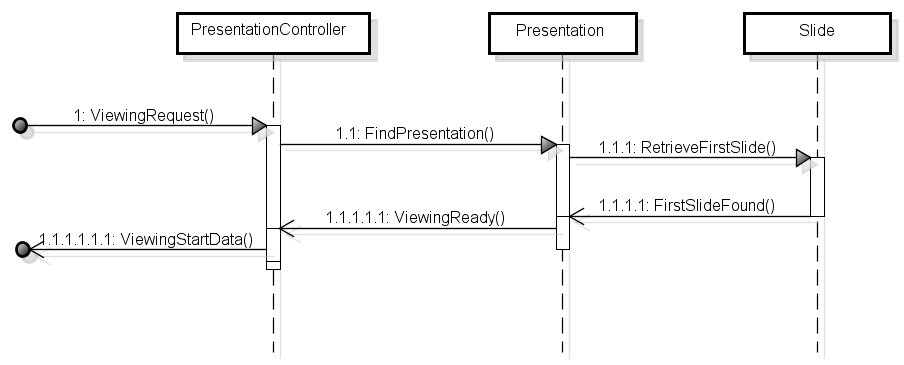
\includegraphics[scale=0.5]{img/view.png}
		\caption{Diagrammi di sequenza - Richiesta di visualizzazione di una presentazione}
	\end{figure} 
	
	
	\subsubsection{Gestione richiesta di creazione di un progetto}
	Il seguente diagramma rappresenta lo scenario con il quale viene gestita una richiesta di creazione di un progetto. La richiesta viene gestita da \textit{ProjectController} il quale crea, tramite CreateProject(), un nuovo progetto in \textit{Project} e invia un ProjectCreatedData() di ritorno.
	
	\begin{figure}[H]
		\centering
		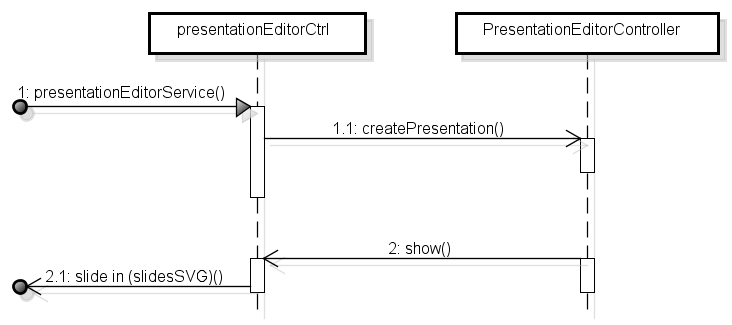
\includegraphics[scale=0.5]{img/create.png}
		\caption{Diagrammi di sequenza - Richiesta di creazione di un progetto}
	\end{figure}
	
\newpage	
	\subsubsection{Gestione richiesta di apertura di un progetto}
	Il seguente diagramma rappresenta lo scenario con il quale viene gestita una richiesta di apertura di un progetto. La richiesta viene gestita da \textit{ProjectController} che invia un SearchForProject() a \textit{Project} per cercare il progetto richiesto. Se l'utente non interrompe l'apertura, da \textit{Project} viene inviato un ProjectFound() a \textit{ProjectController} che ritorna un OpeningProjectData(), altrimenti \textit{Project} invia un OpeningCancelled() e successivamente viene ritornato un UserInterruptMessage() da \textit{ProjectController}.
	
	\begin{figure}[H]
		\centering
		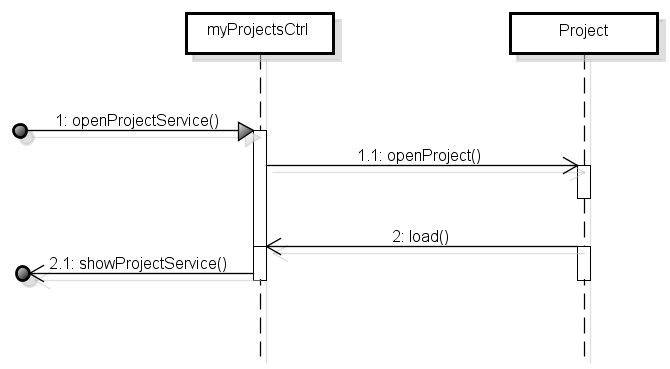
\includegraphics[scale=0.5]{img/open.png}
		\caption{Diagrammi di sequenza - Richiesta di apertura di un progetto}
	\end{figure}
	
	\newpage
	
	\subsubsection{Gestione richiesta di modifica di un progetto}
	Si é deciso di suddividere in sotto-diagrammi il diagramma riguardante la richiesta di modifica, al fine di rendere meno complicata e di più facile comprensione il diagramma stesso. A causa di questa suddivisione i diagrammi saranno tra loro molto simili, la gestione delle richieste infatti é la stessa, cambiano i componenti e il nome di alcuni segnali. Si utilizzerà la dicitura \{element\} per indicare uno degli elementi modificabili di una \gls{slide} (chart, table, image, text, o \gls{real time}) nella seguente spiegazione. 
	\\Lo scenario generale con il quale vengono gestite le richieste é il seguente:
	\begin{itemize}
		\item[]la richiesta di modifica viene gestita da \textit{\{element\}Controller} che la interpreta e invia un InterpretRequest() a \textit{ComponentController}. Nel caso riguardi la creazione di un nuovo \{element\}, \textit{ComponentController} invia un Insert\{element\}() o un Create\{element\}() a \textit{\{element\}} che crea l'elemento richiesto. Viene poi inviato un CreationDone() da \textit{ComponentController} a \textit{\{element\}Controller} che ritorna un ElDataSend().\\
		Se invece la richiesta é una richiesta di modifica \textit{ComponentController} invia un Modify\{element\} a \textit{\{element\}} che può accettare le modifiche con un \{element\}Updated() o rifiutarle con \{element\}Error(). Se vengono accettate \textit{ComponentController} invia un ModifyDone() a \textit{\{element\}Controller} che ritorna un ElDataSend(), altrimenti invia un ModifyError() e viene ritornato un MessageError().
	\end{itemize}
	I diagrammi verranno elencati ora uno dopo l'altro.
	\newpage
	
	\begin{figure}[H]
		\centering
		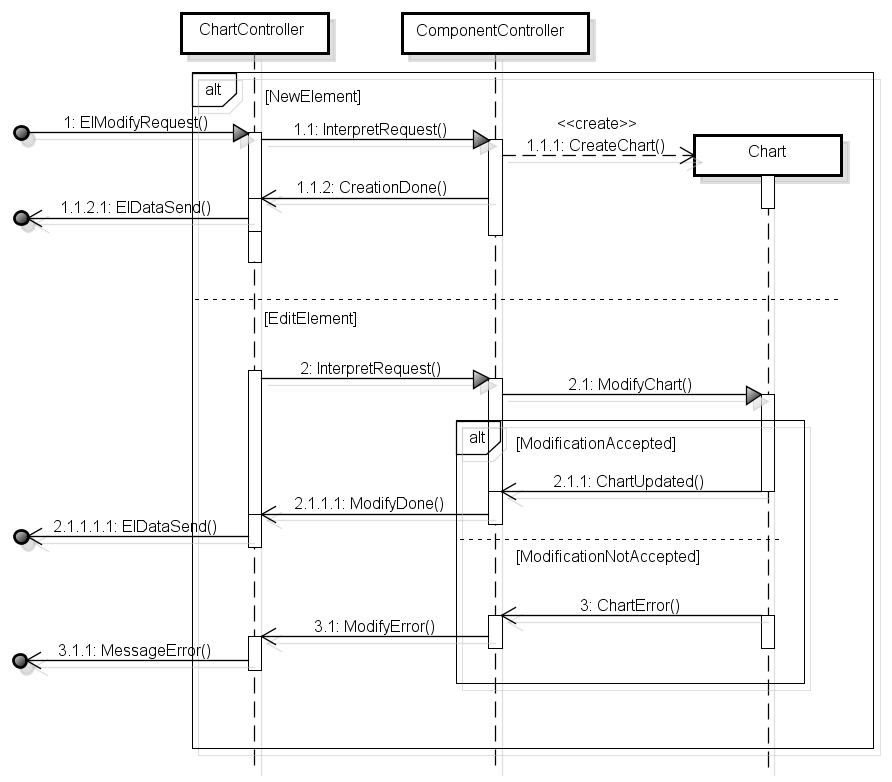
\includegraphics[scale=0.5]{img/chart.png}
		\caption{Diagrammi di sequenza - Richiesta di modifica di un progetto: grafici}
	\end{figure}
	
	\begin{figure}[H]
		\centering
		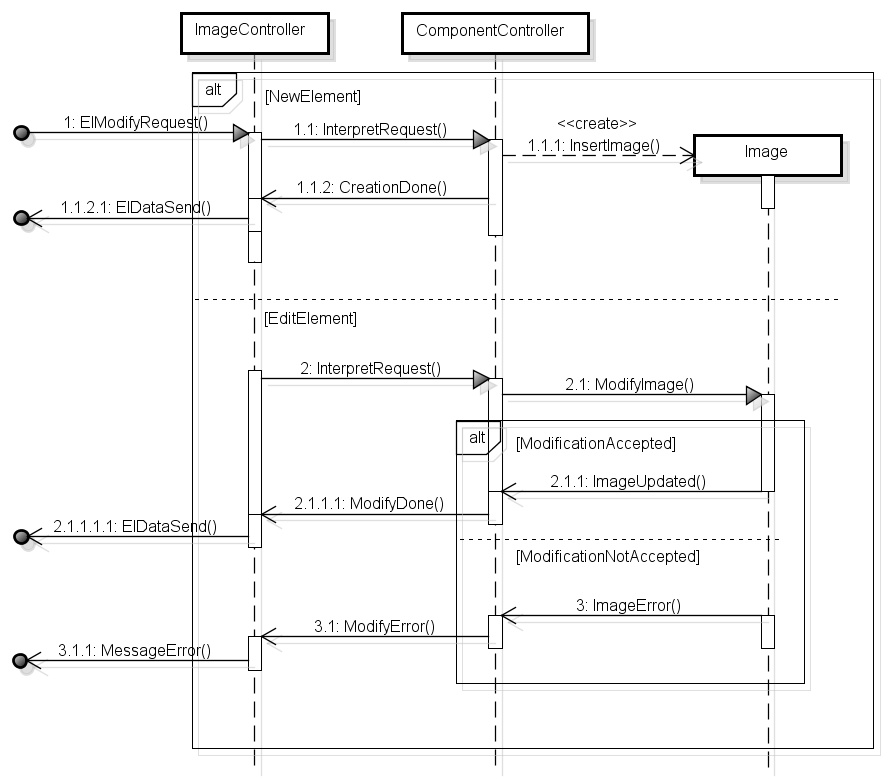
\includegraphics[scale=0.5]{img/image.png}
		\caption{Diagrammi di sequenza - Richiesta di modifica di un progetto: immagini}
	\end{figure}
	
	\begin{figure}[H]
		\centering
		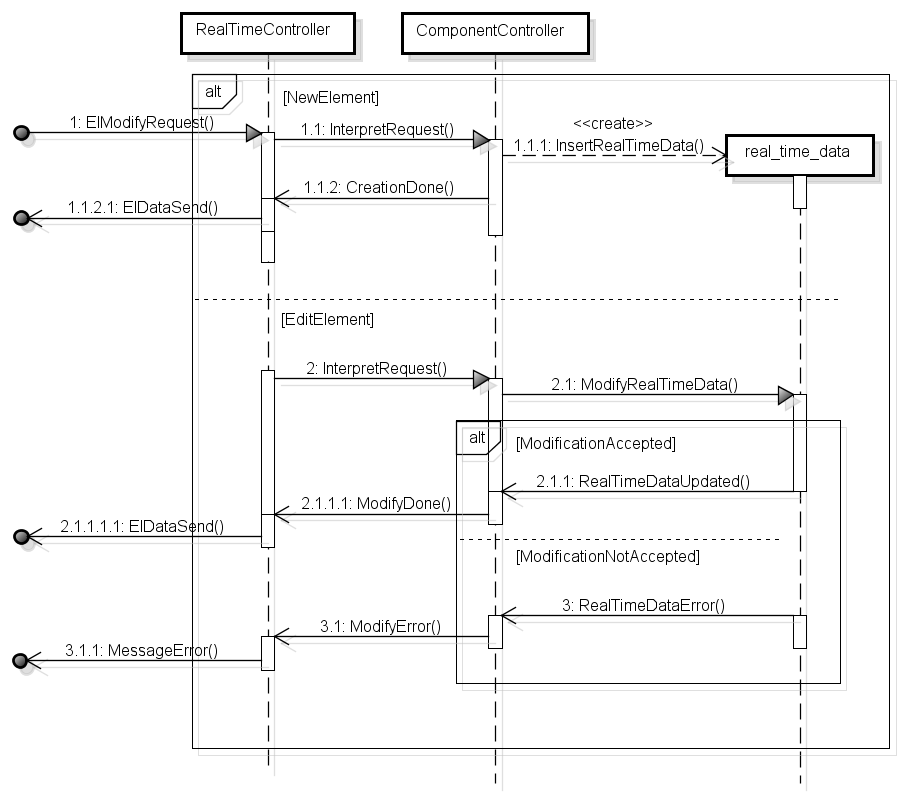
\includegraphics[scale=0.5]{img/real_time.png}
		\caption{Diagrammi di sequenza - Richiesta di modifica di un progetto: dati \gls{Real Time}}
	\end{figure}
	
	\begin{figure}[H]
		\centering
		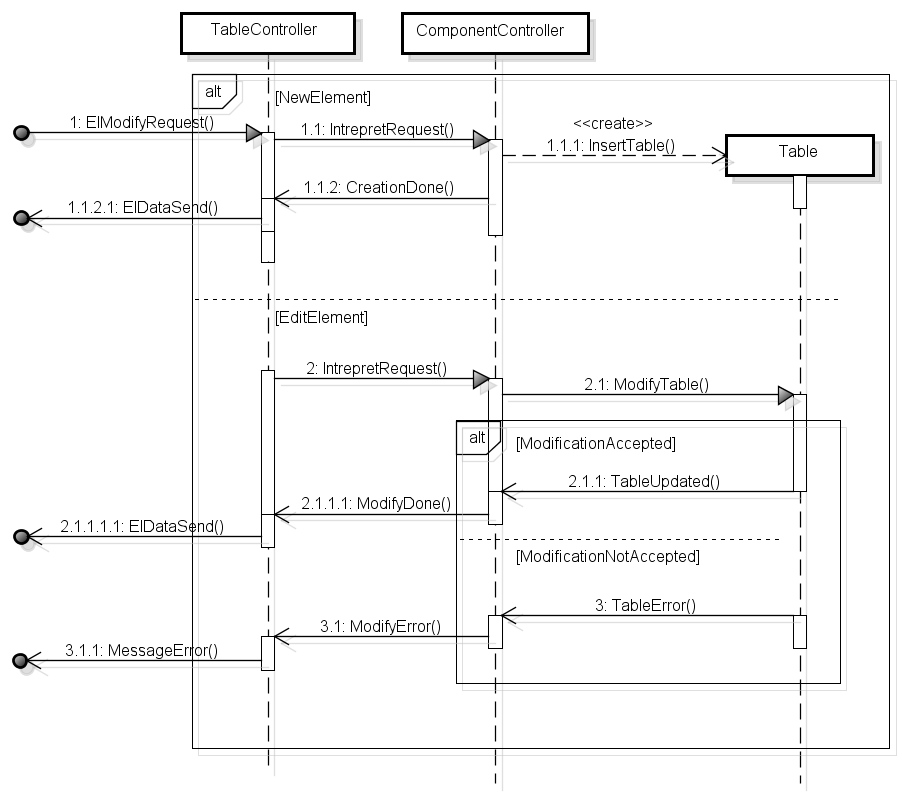
\includegraphics[scale=0.5]{img/table.png}
		\caption{Diagrammi di sequenza - Richiesta di modifica di un progetto: tabelle}
	\end{figure}
	
	\begin{figure}[H]
		\centering
		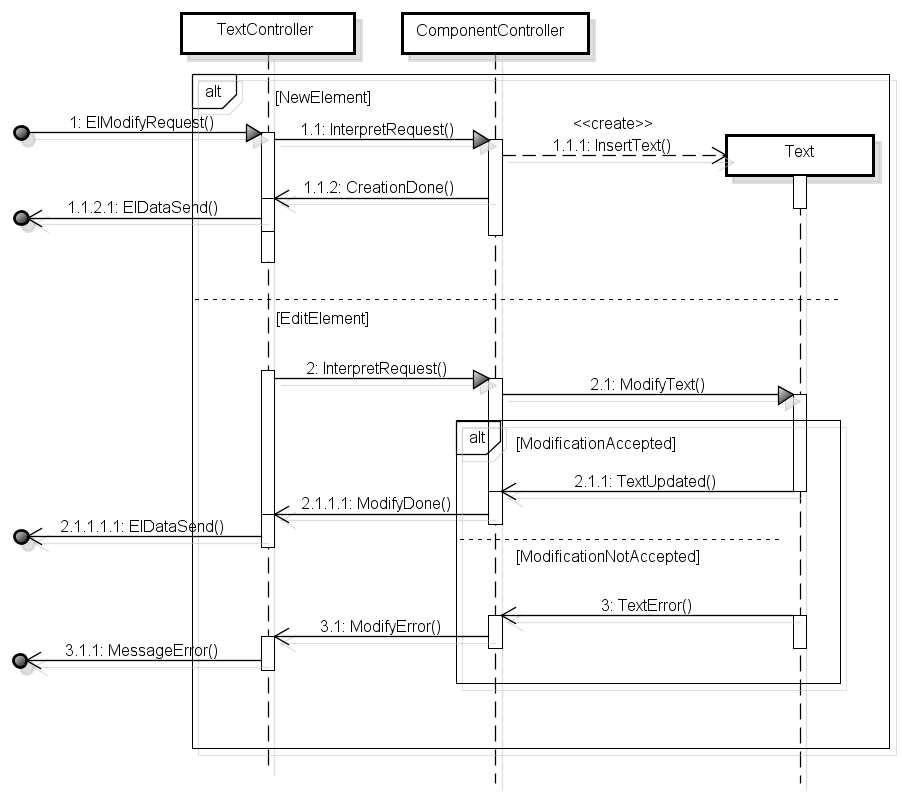
\includegraphics[scale=0.5]{img/text.png}
		\caption{Diagrammi di sequenza - Richiesta di modifica di un progetto: testi}
	\end{figure}
	
	\subsubsection{Gestione richiesta salvataggio di un progetto}
	Il seguente diagramma rappresenta lo scenario con il quale viene gestita una richiesta di salvataggio di un progetto. La richiesta viene gestita da \textit{ProjectController} che invia un SavingProject() a \textit{Project}. Nel caso l'utente confermi il salvataggio viene inviato un ProjectSaved() a \textit{ProjectController} a sua volta invia un SavingData(); se l'utente interrompe il salvataggio \textit{Project} invia un SavingCancelled() a \textit{ProjectController} che ritorna un UserInterruptMessage().
	
	\begin{figure}[H]
		\centering
		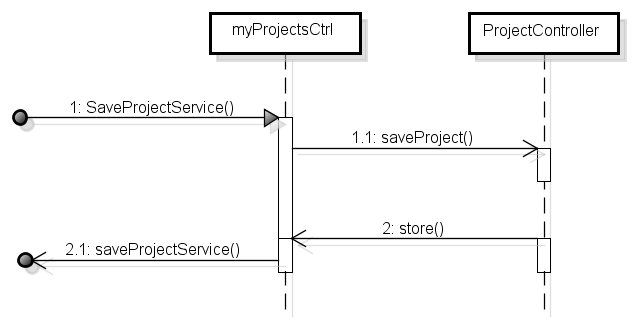
\includegraphics[scale=0.5]{img/save.png}
		\caption{Diagrammi di sequenza - Richiesta di salvataggio di un progetto}
	\end{figure}
	\newpage
